\documentclass[10pt,aspectratio=169]{beamer}
\usepackage[utf8]{inputenc}
\usepackage{listings}
\usepackage{hyperref}
\usepackage{xcolor}
\usepackage{ragged2e}
\usepackage{graphicx}
\usepackage{tikz}
\usetikzlibrary{positioning,calc,decorations.pathreplacing}

\usetheme{Dresden}
%\usetheme{Bergen}

\title{Programming Techniques 2026--2027}
\author{Hannu Parviainen}
\institute{Universidad de la Laguna}
\date{\today}

\lstset{
  language=fortran,
  basicstyle=\ttfamily\scriptsize,
  columns=fullflexible,
  keepspaces=true,
  backgroundcolor=\color{white},
  keywordstyle=\color{blue},
  commentstyle=\color{gray},
  stringstyle=\color{red},
  showstringspaces=false,
  breaklines=true,
  frame=lines
}

\subtitle{Lecture 11: The Barnes--Hut Algorithm}

\begin{document}

\begin{frame}
  \titlepage
\end{frame}


\section{Problem}

\begin{frame}
  \frametitle{The problem: the direct sum scales as $O(N^2)$}
  \begin{columns}[T]
    \begin{column}{0.6\textwidth}
      \begin{itemize}
        \item Every particle feels the gravity of every other particle, so the direct sum of Exercise 1 computes the force between every pair of particles.
        \item With $N$ particles, there are $\frac{1}{2}N(N-1)$ pairs:

          \vspace*{1mm}
          \centering
          \small
          \begin{tabular}{rr}
            $N$ & pairs \\
            \hline
            2 & 1 \\
            3 & 3 \\
            4 & 6 \\
            10 & 45 \\
            100 & 4\,950 \\
            1000 & 499\,500 \\
          \end{tabular}

        \item For large $N$, $\frac{1}{2}N(N-1) \approx \frac{1}{2}N^2$, so the run time grows as $N^2$. We say that the direct sum scales as $O(N^2)$.
      \end{itemize}
    \end{column}

    \begin{column}{0.4\textwidth}
      \centering
      \vspace*{4mm}
      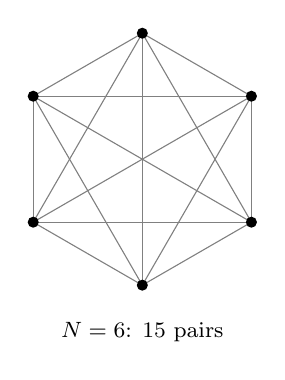
\begin{tikzpicture}
        \foreach \i in {0,...,5} {
          \coordinate (p\i) at ({90 + 60*\i}:1.6);
        }
        \foreach \i in {0,...,5} {
          \foreach \j in {0,...,5} {
            \ifnum\i<\j \draw[gray] (p\i) -- (p\j); \fi
          }
        }
        \foreach \i in {0,...,5} {
          \fill (p\i) circle[radius=2pt];
        }
        \node[font=\footnotesize] at (0,-2.2) {$N = 6$: 15 pairs};
      \end{tikzpicture}
    \end{column}
  \end{columns}
\end{frame}


\begin{frame}
  \frametitle{Computational scaling}
  \begin{columns}[T]
    \begin{column}{0.5\textwidth}
      \begin{itemize}
        \item If the run time $T$ grows as $N^2$, ten times more particles take a hundred times longer.
        \item<2-> \textbf{Not good!}
        \item<3-> \textbf{Not good at all!} If $N = 1000$ takes one second, $N = 10^6$ takes $10^6$ seconds, almost 12 days.
        \item<4-> What can we do? \textbf{The Barnes--Hut algorithm} scales as $O(N \log N)$, and $N = 10^6$ takes about half an hour. \\
          {\footnotesize J. Barnes and P. Hut (1986), \emph{A hierarchical $O(N \log N)$ force-calculation algorithm}, Nature 324, 446--449.}
      \end{itemize}
    \end{column}

    \begin{column}{0.5\textwidth}
      \centering
      \vspace*{2mm}
      \small
      \begin{tabular}{lrr}
        & $T \propto N^2$ & \uncover<4->{$T \propto N \log N$} \\
        \hline
        \( T_{N=100} / T_{N=10} \)             & 100       & \uncover<4->{20} \\
        \( T_{N=1000} / T_{N=100} \)           & 100       & \uncover<4->{15} \\
        \( T_{N=10\,000} / T_{N=1000} \)       & 100       & \uncover<4->{13.3} \\
        \( T_{N=10\,000} / T_{N=10} \)         & $10^6$    & \uncover<4->{4000} \\
        \hline
      \end{tabular}
    \end{column}
  \end{columns}
\end{frame}


\section{Idea}

\begin{frame}
  \centering
  \Huge \textbf{How?}

  \pause
  \vspace*{5mm}
  \Large Treat a distant group of particles as a single point mass at its centre of mass.
\end{frame}


\begin{frame}
  \frametitle{Barnes--Hut: group the distant particles}
  \begin{columns}[T]
    \begin{column}{0.5\textwidth}
      \centering
      \begin{tikzpicture}[x=1cm, y=1cm]
        % A group of five particles (a) and a pair (b), with equal masses
        \coordinate (a1) at (3.55,3.95);
        \coordinate (a2) at (4.05,3.75);
        \coordinate (a3) at (3.70,3.35);
        \coordinate (a4) at (4.20,3.20);
        \coordinate (a5) at (3.40,3.10);
        \coordinate (b1) at (0.90,1.20);
        \coordinate (b2) at (1.55,0.85);
        \coordinate (A) at (3.78,3.47);    % centre of mass of the group
        \coordinate (B) at (1.225,1.025);  % centre of mass of the pair

        \draw (0,0) rectangle (5,5);

        % 2: the direct sum, every pair
        \only<2>{
          \foreach \p/\q in {a1/a2, a1/a3, a1/a4, a1/a5, a2/a3, a2/a4, a2/a5, a3/a4, a3/a5, a4/a5,
                             b1/b2, a1/b1, a2/b1, a3/b1, a4/b1, a5/b1, a1/b2, a2/b2, a3/b2, a4/b2, a5/b2} {
            \draw[gray] (\p) -- (\q);
          }
        }

        % 3: seen from the pair, the group is one point mass
        \only<3>{
          \fill[blue!20] (A) circle[radius=0.78];
          \draw[gray] (b1) -- (b2);
          \draw[blue, thick] (b1) -- (A) (b2) -- (A);
          \draw[blue, thick] (A) +(-3pt,-3pt) -- +(3pt,3pt) +(-3pt,3pt) -- +(3pt,-3pt);
          \node[blue, right, font=\footnotesize] at (4.56,3.47) {$M$};
        }

        % 4: seen from the group, the pair is one point mass
        \only<4>{
          \fill[blue!20] (B) circle[radius=0.55];
          \foreach \p/\q in {a1/a2, a1/a3, a1/a4, a1/a5, a2/a3, a2/a4, a2/a5, a3/a4, a3/a5, a4/a5} {
            \draw[gray] (\p) -- (\q);
          }
          \foreach \p in {a1, a2, a3, a4, a5} {
            \draw[blue, thick] (\p) -- (B);
          }
          \draw[blue, thick] (B) +(-3pt,-3pt) -- +(3pt,3pt) +(-3pt,3pt) -- +(3pt,-3pt);
          \node[blue, below, font=\footnotesize] at (1.225,0.475) {$M'$};
        }

        \foreach \p in {a1, a2, a3, a4, a5, b1, b2} {
          \fill (\p) circle[radius=2pt];
        }
      \end{tikzpicture}
    \end{column}

    \begin{column}{0.5\textwidth}
      \only<1>{
        Seven particles of equal mass: a group of five, and a pair far away from it.
      }
      \only<2>{
        \textbf{Direct sum:} the force between every pair, $\frac{1}{2} \cdot 7 \cdot 6 = 21$ pairs. Each particle needs 6 terms.
      }
      \only<3>{
        \textbf{Seen from the pair}, the group is far away. Its pull is almost the same as that of one particle with the group's total mass $M$ at its centre of mass.

        \vspace*{2mm}
        Each particle of the pair needs 2 terms instead of 6.
      }
      \only<4>{
        \textbf{Seen from the group}, the pair is far away too, and acts as one point mass $M'$.

        \vspace*{2mm}
        The particles of the group are close to each other, so they still interact directly. Each needs 5 terms instead of 6.

        \vspace*{2mm}
        With many particles, most of the others are far away, and the saving is much larger.
      }
    \end{column}
  \end{columns}
\end{frame}


\begin{frame}
  \frametitle{When is a group far enough? The opening angle $\theta$}
  \begin{columns}[T]
    \begin{column}{0.45\textwidth}
      \centering
      \vspace*{4mm}
      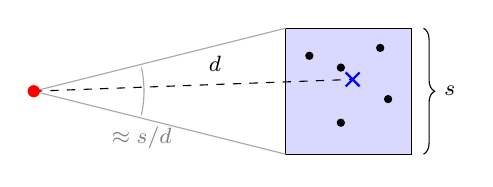
\begin{tikzpicture}[x=1cm, y=1cm]
        \coordinate (P) at (0,0);
        \coordinate (C) at (4.05,0.15);   % centre of mass of the node
        % The box: a square of side s
        \fill[blue!15] (3.2,-0.8) rectangle (4.8,0.8);
        \draw (3.2,-0.8) rectangle (4.8,0.8);
        \foreach \x/\y in {3.5/0.45, 3.9/-0.4, 4.4/0.55, 4.5/-0.1, 3.9/0.3} {
          \fill (\x,\y) circle[radius=1.5pt];
        }
        % The angle at which the node is seen from the particle
        \draw[gray!70] (P) -- (3.2,0.8) (P) -- (3.2,-0.8);
        \draw[gray!70] (12.5:1.4) arc[start angle=12.5, end angle=-12.5, radius=1.4];
        \node[gray, below, font=\footnotesize] at (1.37,-0.33) {$\approx s/d$};
        % Distance and size
        \draw[dashed] (P) -- (C);
        \node[above, font=\footnotesize] at (2.3,0.12) {$d$};
        \draw[blue, thick] (C) +(-2.5pt,-2.5pt) -- +(2.5pt,2.5pt) +(-2.5pt,2.5pt) -- +(2.5pt,-2.5pt);
        \draw[decorate, decoration={brace, amplitude=4pt}] (4.95,0.8) -- (4.95,-0.8) node[midway, right=4pt, font=\footnotesize] {$s$};
        \fill[red] (P) circle[radius=2.2pt];
      \end{tikzpicture}
    \end{column}

    \begin{column}{0.55\textwidth}
      \begin{itemize}
        \item A group inside a box of size $s$, whose centre of mass is at distance $d$, is used as a single point mass if $s / d < \theta$.
        \item $s/d$ is roughly the angle at which the box is seen from the particle, so $\theta$ is called the \emph{opening angle}.
        \item A smaller $\theta$ is more accurate but slower. With $\theta = 0$, no group is a point mass, and we get the direct sum.
        \item Typical values are $\theta \approx 0.5$--$1$. Exercise 2 uses $\theta = 0.5$.
        \item To find the groups quickly, we organise the particles in a tree.
      \end{itemize}
    \end{column}
  \end{columns}
\end{frame}


\section{Octrees}

\begin{frame}
  \centering
  \Huge \textbf{Octrees}
\end{frame}


\begin{frame}
  \frametitle{Quadtrees and octrees}
  \begin{columns}[T]
    \begin{column}{0.45\textwidth}
      \begin{itemize}
        \item A \textbf{quadtree} divides a square into four smaller squares, and those into four again, as many times as needed.
        \item An \textbf{octree} does the same in 3D: it divides a cube into eight smaller cubes.
        \item Each node of the tree is a square (or a cube). Its children are its four quarters (or eight octants).
        \item The \textbf{root} contains all the particles. A \textbf{leaf} is a node without children.
        \item In the Barnes--Hut tree, a leaf holds at most one particle.
      \end{itemize}
    \end{column}

    \begin{column}{0.55\textwidth}
      \centering
      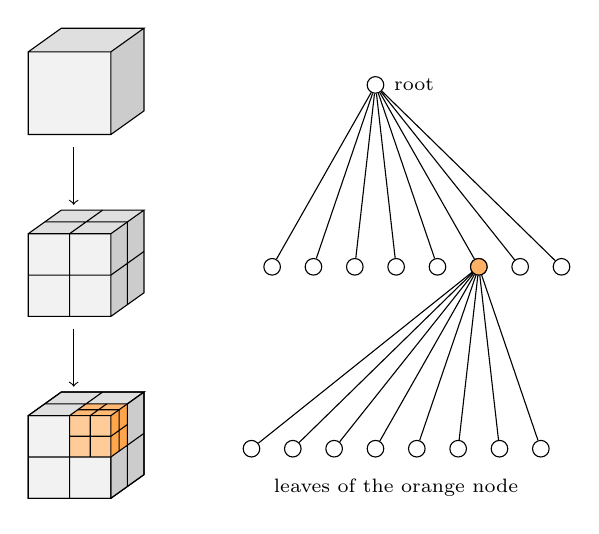
\begin{tikzpicture}[x=1.05cm, y=1.05cm, z={(0.42cm,0.3cm)},
          cube/.pic={
            \fill[gray!10] (0,0,0) -- (1,0,0) -- (1,1,0) -- (0,1,0) -- cycle;
            \fill[gray!25] (0,1,0) -- (1,1,0) -- (1,1,1) -- (0,1,1) -- cycle;
            \fill[gray!40] (1,0,0) -- (1,0,1) -- (1,1,1) -- (1,1,0) -- cycle;
            \draw (0,0,0) -- (1,0,0) -- (1,1,0) -- (0,1,0) -- cycle
                  (0,1,0) -- (0,1,1) -- (1,1,1) -- (1,1,0)
                  (1,0,0) -- (1,0,1) -- (1,1,1);
          },
          tnode/.style={circle, draw, fill=white, inner sep=0pt, minimum size=6pt}]

        % Level 0: one cube
        \pic at (0,4.4,0) {cube};

        % Level 1: the cube divided into eight
        \begin{scope}[shift={(0,2.2,0)}]
          \pic {cube};
          \draw (0.5,0,0) -- (0.5,1,0) (0,0.5,0) -- (1,0.5,0)
                (0.5,1,0) -- (0.5,1,1) (0,1,0.5) -- (1,1,0.5)
                (1,0.5,0) -- (1,0.5,1) (1,0,0.5) -- (1,1,0.5);
        \end{scope}

        % Level 2: one octant divided again
        \begin{scope}[shift={(0,0,0)}]
          \pic {cube};
          \fill[orange!40] (0.5,0.5,0) rectangle (1,1,0);
          \fill[orange!55] (0.5,1,0) -- (1,1,0) -- (1,1,0.5) -- (0.5,1,0.5) -- cycle;
          \fill[orange!70] (1,0.5,0) -- (1,1,0) -- (1,1,0.5) -- (1,0.5,0.5) -- cycle;
          \draw (0,0,0) -- (1,0,0) -- (1,1,0) -- (0,1,0) -- cycle
                (0,1,0) -- (0,1,1) -- (1,1,1) -- (1,1,0)
                (1,0,0) -- (1,0,1) -- (1,1,1);
          \draw (0.5,0,0) -- (0.5,1,0) (0,0.5,0) -- (1,0.5,0)
                (0.5,1,0) -- (0.5,1,1) (0,1,0.5) -- (1,1,0.5)
                (1,0.5,0) -- (1,0.5,1) (1,0,0.5) -- (1,1,0.5);
          \draw (0.75,0.5,0) -- (0.75,1,0) (0.5,0.75,0) -- (1,0.75,0)
                (0.75,1,0) -- (0.75,1,0.5) (0.5,1,0.25) -- (1,1,0.25)
                (1,0.75,0) -- (1,0.75,0.5) (1,0.5,0.25) -- (1,1,0.25);
        \end{scope}

        \draw[->] (0.55,4.25) -- (0.55,3.55);
        \draw[->] (0.55,2.05) -- (0.55,1.35);

        % The tree, one level next to each cube
        \node[tnode] (root) at (4.2,5.0) {};
        \foreach \i in {1,...,8} {
          \node[tnode] (c\i) at ({2.45 + 0.5*\i},2.8) {};
          \draw (root) -- (c\i);
        }
        \node[tnode, fill=orange!60] at (c6) {};
        \foreach \j in {1,...,8} {
          \node[tnode] (g\j) at ({2.2 + 0.5*\j},0.6) {};
          \draw (c6) -- (g\j);
        }
        \node[font=\scriptsize, anchor=west] at (root.east) {root};
        \node[font=\scriptsize, anchor=north] at (4.45,0.35) {leaves of the orange node};
      \end{tikzpicture}
    \end{column}
  \end{columns}
\end{frame}


\begin{frame}
  \frametitle{Building a quadtree}
  \begin{columns}[T]
    \begin{column}{0.5\textwidth}
      \centering
      \input{quadtree_build}
    \end{column}

    \begin{column}{0.5\textwidth}
      \begin{itemize}
        \item The figure shows a quadtree, but an octree works in the same way.
        \item The root covers all the particles. Exercise 2 makes it 0.1\,\% larger than needed, so that no particle lies exactly on its edge.
        \item The figure divides the nodes level by level. The algorithm inserts the particles one at a time, but the final tree is the same whatever the order.
        \item Dense regions get small nodes, and empty regions stay large.
        \item For evenly spread particles, the depth of the tree grows as $\log N$.
      \end{itemize}
    \end{column}
  \end{columns}
\end{frame}


\begin{frame}
  \frametitle{Inserting a particle}
  \begin{columns}[T]
    \begin{column}{0.55\textwidth}
      Start from the root, and go down the tree:
      \begin{enumerate}
        \item An \textbf{empty node} gets the particle.
        \item A \textbf{leaf with a particle} is divided into eight children. Its old particle moves to the child that contains it, and the new particle continues as in case 3.
        \item A \textbf{node with children} passes the particle on to the child that contains it.
      \end{enumerate}

      \vspace*{2mm}
      \begin{itemize}
        \item Every node on the way adds one to its count of particles.
        \item Two particles at the same position would be divided forever, so the depth of the tree is limited to \texttt{max\_depth}.
      \end{itemize}
    \end{column}

    \begin{column}{0.45\textwidth}
      \centering
      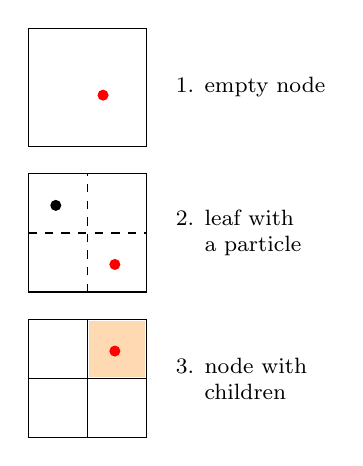
\begin{tikzpicture}[x=1cm, y=1cm, font=\footnotesize]
        % 1: an empty node
        \draw (0,3.1) rectangle (1.5,4.6);
        \fill[red] (0.95,3.75) circle[radius=2pt];
        \node[anchor=west, align=left] at (1.75,3.85) {1. empty node};

        % 2: a leaf with a particle
        \draw (0,1.25) rectangle (1.5,2.75);
        \draw[dashed] (0.75,1.25) -- (0.75,2.75) (0,2.0) -- (1.5,2.0);
        \fill (0.35,2.35) circle[radius=2pt];
        \fill[red] (1.1,1.6) circle[radius=2pt];
        \node[anchor=west, align=left] at (1.75,2.0) {2. leaf with \\ \phantom{2. }a particle};

        % 3: a node with children
        \draw (0,-0.6) rectangle (1.5,0.9) (0.75,-0.6) -- (0.75,0.9) (0,0.15) -- (1.5,0.15);
        \fill[orange!30] (0.77,0.17) rectangle (1.48,0.88);
        \fill[red] (1.1,0.5) circle[radius=2pt];
        \node[anchor=west, align=left] at (1.75,0.15) {3. node with \\ \phantom{3. }children};
      \end{tikzpicture}
    \end{column}
  \end{columns}
\end{frame}


\begin{frame}[fragile]
  \frametitle{The octree node}
  \begin{columns}[T]
    \begin{column}{0.5\textwidth}
      \centering
      \vspace*{2mm}
      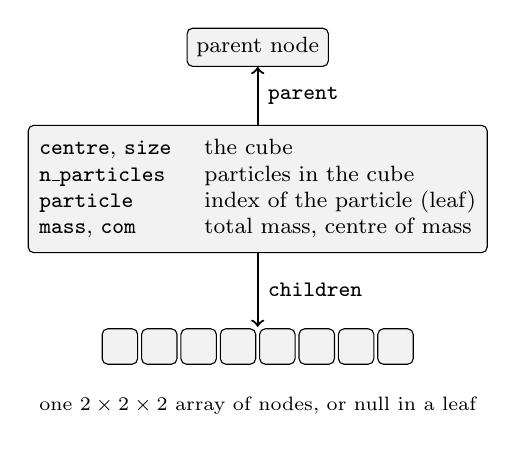
\begin{tikzpicture}[x=1cm, y=1cm, font=\footnotesize,
          box/.style={draw, fill=gray!10, rounded corners=2pt}]
        \node[box, inner sep=4pt] (nd) at (0,0) {
          \begin{tabular}{@{}ll@{}}
            \texttt{centre}, \texttt{size} & the cube \\
            \texttt{n\_particles} & particles in the cube \\
            \texttt{particle} & index of the particle (leaf) \\
            \texttt{mass}, \texttt{com} & total mass, centre of mass \\
          \end{tabular}
        };
        \node[box, minimum width=1.6cm] (parent) at (0,1.8) {parent node};
        \draw[->, thick] (nd.north) -- (parent.south) node[midway, right] {\texttt{parent}};

        \foreach \i in {1,...,8} {
          \node[box, minimum size=0.45cm] (ch\i) at ({-2.25 + 0.5*\i},-2.0) {};
        }
        \draw[->, thick] (nd.south) -- (0,-1.75) node[midway, right] {\texttt{children}};
        \node[align=center, font=\scriptsize] at (0,-2.75) {one $2 \times 2 \times 2$ array of nodes, or null in a leaf};
      \end{tikzpicture}
    \end{column}

    \begin{column}{0.5\textwidth}
      \begin{lstlisting}
type :: node
  real(dp) :: centre(3)   ! centre of the cube
  real(dp) :: size        ! side length of the cube
  integer :: n_particles = 0
  integer :: particle = 0 ! the particle in a leaf
  real(dp) :: mass = 0.0_dp
  real(dp) :: com(3) = 0.0_dp  ! centre of mass
  type(node), pointer :: parent => null()
  type(node), pointer :: &
      children(:,:,:) => null()
end type node
      \end{lstlisting}
      \small
      The eight children are allocated together, as one array, when a node is divided. The particles stay in the particle arrays of the main program, and a leaf stores only the index of its particle.
    \end{column}
  \end{columns}
\end{frame}


\section{Forces}

\begin{frame}
  \centering
  \Huge \textbf{Forces}
\end{frame}


\begin{frame}
  \frametitle{Mass and centre of mass, from the leaves up}
  \begin{columns}[T]
    \begin{column}{0.5\textwidth}
      \begin{itemize}
        \item A leaf has the mass and position of its particle.
        \item A node with children gets its total mass $M$ and centre of mass $\mathbf{R}$ from its children $c$:
          \[ M = \sum_c M_c, \qquad \mathbf{R} = \frac{1}{M} \sum_c M_c \mathbf{R}_c. \]
        \item A recursive procedure first calls itself for each child, and only then combines the results, so the children are always computed before their parent.
        \item Empty nodes have zero mass and are skipped.
      \end{itemize}
    \end{column}

    \begin{column}{0.5\textwidth}
      \centering
      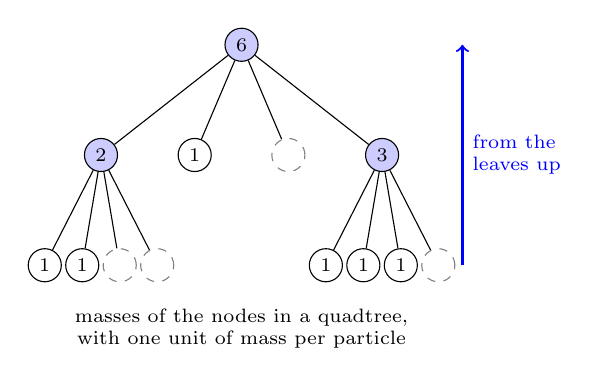
\begin{tikzpicture}[x=0.85cm, y=1cm, font=\scriptsize,
          tnode/.style={circle, draw, fill=white, inner sep=0pt, minimum size=4.2mm},
          empty/.style={circle, draw, dashed, gray, inner sep=0pt, minimum size=4.2mm}]
        \node[tnode, fill=blue!20] (root) at (0,0) {6};
        \node[tnode, fill=blue!20] (a) at (-2.1,-1.4) {2};
        \node[tnode] (b) at (-0.7,-1.4) {1};
        \node[empty] (c) at (0.7,-1.4) {};
        \node[tnode, fill=blue!20] (d) at (2.1,-1.4) {3};
        \foreach \n in {a, b, c, d} { \draw (root) -- (\n); }
        \foreach \dx/\s in {-0.84/tnode, -0.28/tnode, 0.28/empty, 0.84/empty} {
          \node[\s] (x) at ({-2.1 + \dx},-2.8) {};
          \draw (a) -- (x);
        }
        \foreach \dx/\s in {-0.84/tnode, -0.28/tnode, 0.28/tnode, 0.84/empty} {
          \node[\s] (y) at ({2.1 + \dx},-2.8) {};
          \draw (d) -- (y);
        }
        \foreach \x in {-2.94, -2.38, 1.26, 1.82, 2.38} {
          \node at (\x,-2.8) {1};
        }
        \draw[->, thick, blue] (3.3,-2.8) -- (3.3,0) node[midway, right, align=left] {from the \\ leaves up};
        \node[align=center] at (0,-3.6) {masses of the nodes in a quadtree, \\ with one unit of mass per particle};
      \end{tikzpicture}
    \end{column}
  \end{columns}
\end{frame}


\begin{frame}[fragile]
  \frametitle{The pull of a point mass}
  \begin{columns}[T]
    \begin{column}{0.42\textwidth}
      \begin{itemize}
        \item Single particles and point masses pull with the same formula. A mass $m$ at the relative position $\mathbf{d}$, softened with the length $\epsilon$, gives
          \[ \mathbf{a} = \frac{m \mathbf{d}}{(|\mathbf{d}|^2 + \epsilon^2)^{3/2}}. \]
        \item With $\epsilon = 0$, this is Newton's gravity with $G = 1$, as in Exercise~1.
        \item Softening keeps the pull finite when two particles pass close to each other. Exercise 2 uses $\epsilon = 0.01$.
      \end{itemize}
    \end{column}

    \begin{column}{0.58\textwidth}
      \begin{lstlisting}
pure function point_mass_acceleration(mass, d) result(acc)
  real(dp), intent(in) :: mass, d(3)
  real(dp) :: acc(3)
  acc = mass * d / (sum(d**2) + eps**2)**1.5_dp
end function point_mass_acceleration
      \end{lstlisting}

      \centering
      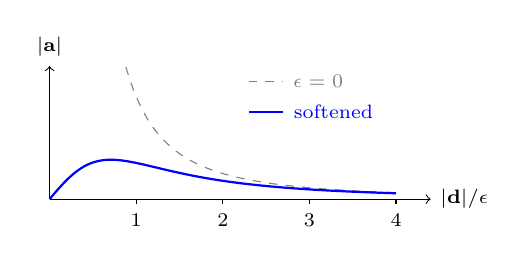
\begin{tikzpicture}[x=1.1cm, y=1.3cm, font=\scriptsize]
        \draw[->] (0,0) -- (4.4,0) node[right] {$|\mathbf{d}| / \epsilon$};
        \draw[->] (0,0) -- (0,1.3) node[above] {$|\mathbf{a}|$};
        \foreach \x in {1,2,3,4} {
          \draw (\x,0) -- (\x,-0.05) node[below] {\x};
        }
        \draw[gray, dashed, domain=0.88:4, samples=60] plot (\x, {1/(\x*\x)});
        \draw[blue, thick, domain=0:4, samples=80] plot (\x, {\x/((\x*\x + 1)^1.5)});
        % Legend
        \draw[gray, dashed] (2.3,1.15) -- ++(0.4,0) node[right] {$\epsilon = 0$};
        \draw[blue, thick] (2.3,0.85) -- ++(0.4,0) node[right] {softened};
      \end{tikzpicture}
    \end{column}
  \end{columns}
\end{frame}


\begin{frame}
  \frametitle{Walking the tree}
  \begin{columns}[T]
    \begin{column}{0.42\textwidth}
      The acceleration of particle \texttt{i} is a sum over a walk down the tree, starting from the root:
      \begin{itemize}
        \item An \textbf{empty node} adds nothing.
        \item A \textbf{leaf} adds the pull of its particle, unless it is particle \texttt{i} itself.
        \item A \textbf{node far enough away}, with $s < \theta d$, adds the pull of a point mass at its centre of mass.
        \item Any \textbf{other node} is opened: visit its children.
      \end{itemize}
    \end{column}

    \begin{column}{0.58\textwidth}
      \centering
      \vspace*{2mm}
      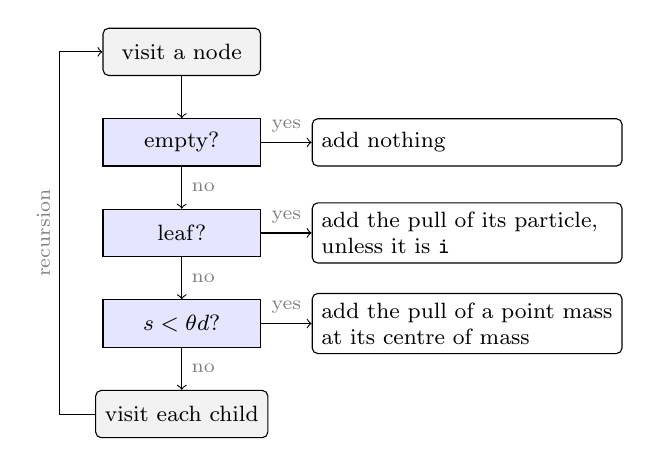
\begin{tikzpicture}[font=\footnotesize,
          stage/.style={draw, rounded corners=2pt, fill=gray!10, align=center, minimum width=20mm, minimum height=6mm},
          test/.style={draw, fill=blue!10, align=center, minimum width=20mm, minimum height=6mm},
          act/.style={draw, rounded corners=2pt, align=left, text width=37mm, minimum height=6mm},
          lab/.style={font=\scriptsize, gray}]
        \node[stage] (visit) at (0,0) {visit a node};
        \node[test] (empty) at (0,-1.15) {empty?};
        \node[test] (leaf) at (0,-2.3) {leaf?};
        \node[test] (far) at (0,-3.45) {$s < \theta d$?};
        \node[stage] (open) at (0,-4.6) {visit each child};
        \node[act, anchor=west] (a1) at (1.65,-1.15) {add nothing};
        \node[act, anchor=west] (a2) at (1.65,-2.3) {add the pull of its particle, unless it is \texttt{i}};
        \node[act, anchor=west] (a3) at (1.65,-3.45) {add the pull of a point mass at its centre of mass};
        \draw[->] (visit) -- (empty);
        \draw[->] (empty) -- node[lab, right] {no} (leaf);
        \draw[->] (leaf) -- node[lab, right] {no} (far);
        \draw[->] (far) -- node[lab, right] {no} (open);
        \foreach \q/\a in {empty/a1, leaf/a2, far/a3} {
          \draw[->] (\q) -- node[lab, above] {yes} (\a);
        }
        \draw[->] (open.west) -- ++(-0.45,0) |- node[lab, pos=0.25, rotate=90, above] {recursion} (visit.west);
      \end{tikzpicture}
    \end{column}
  \end{columns}
\end{frame}


\begin{frame}
  \frametitle{What one particle sees}
  \begin{columns}[T]
    \begin{column}{0.5\textwidth}
      \centering
      \input{tree_walk}
    \end{column}

    \begin{column}{0.5\textwidth}
      The tree walk of the \textcolor{red}{red particle}, for three opening angles:
      \begin{itemize}
        \item \textcolor{gray}{Grey lines}: particles used directly.
        \item \textcolor{blue}{Blue lines} and shaded nodes: nodes used as point masses, with their centres of mass as crosses.
      \end{itemize}

      \vspace*{2mm}
      \only<1>{With $\theta = 0$, every node is opened, and the walk gives the direct sum.}
      \only<2>{With $\theta = 0.5$, the distant group is replaced by the centres of mass of four nodes.}
      \only<3>{With $\theta = 1$, the whole upper-right quarter is one point mass. The forces are faster to compute, but less accurate.}
    \end{column}
  \end{columns}
\end{frame}


\begin{frame}[fragile]
  \frametitle{One time step}
  \begin{columns}[T]
    \begin{column}{0.45\textwidth}
      \begin{itemize}
        \item The particles move, so the tree is built again after every drift of the leapfrog step.
        \item The tree is deleted after use. Otherwise every step would leak the memory of all its nodes.
        \item \texttt{delete\_children} deallocates the children of a node after deleting their own children, again by recursion.
        \item Building the tree takes $O(N \log N)$ time, and each walk visits $O(\log N)$ nodes, so a step takes $O(N \log N)$ time.
      \end{itemize}
    \end{column}

    \begin{column}{0.55\textwidth}
      \begin{lstlisting}
subroutine compute_accelerations(m, r, a)
  real(dp), intent(in) :: m(:), r(:,:)
  real(dp), intent(out) :: a(:,:)
  type(node), pointer :: root
  integer :: i

  call build_tree(root, r)
  call compute_masses(root, m, r)
  do i = 1, size(m)
    a(:,i) = 0.0_dp
    call add_acceleration(root, i, r, a(:,i))
  end do
  call delete_children(root)
  deallocate(root)
end subroutine compute_accelerations
      \end{lstlisting}
    \end{column}
  \end{columns}
\end{frame}


\section{Summary}

\begin{frame}
  \frametitle{Summary}
  \begin{itemize}
    \item The direct sum scales as $O(N^2)$. The Barnes--Hut algorithm scales as $O(N \log N)$.
    \item It puts the particles into an octree, and treats a node as a single point mass when it is seen at an angle smaller than $\theta$.
    \item Each time step:
      \begin{enumerate}
        \item build the tree,
        \item compute the masses and centres of mass from the leaves up,
        \item walk the tree for each particle,
        \item delete the tree.
      \end{enumerate}
    \item Recursion fits trees well: inserting, computing the masses, walking, and deleting are all short recursive procedures.
  \end{itemize}

  \vspace*{2mm}
  \textbf{Next: Exercise 2} starts from \texttt{lectures/exercise\_2/barnes\_hut.f90}, which implements everything in this lecture. The walk of each particle is independent of the others, so in the exercise you share the particles between MPI processes.
\end{frame}

\end{document}
